\section{Analysis}

\subsection{Background}
There exists online many popular "remixes"  where someone has taken an existing song and distorted it, usually by adjusting its speed, bass and pitch, to achieve a desired effect. Often these versions of the song are preferred to the originals when used to accompany short-form content on video-sharing sites such as TikTok. For example,  the song "Money Trees" by Kendrick Lamar has 120 million views on YouTube  in its original form, but also a sizeable 1.6 million views on one "TikTok remix" alone, and indeed on TikTok itself it is rare to hear the original version. This pattern is also observed on other short-form video content sites, such as Instagram Reels and YouTube Shorts.

\paragraph{}
As such it can be seen that there exists a large audience of people who enjoy listening to altered versions of popular songs. However, the most popular music listening programs, including Spotify and YouTube music, provide no mechanism for manually altering songs by one's self. Instead, "remixes" must be created in external audio editing programs. Thus if a user wants to create their own "remixes", a unique issue is presented:
\begin{itemize}
	\item Suppose, for example, that a user wants to listen to a selection of songs, but sped-up and with a bass-boost applied, as is typical for song "remixes" on TikTok. Many songs do not have any accompanying "remixes" to satisfy this user's need, so they wish to do things themselves.
	\item As there exists no mainstream solution to edit music in real-time, the user would have to import their music files into an audio editing program and apply any desired effects to each file. This will take considerable time.
	\item However, what if the user then wishes to change the intensity or nature of the effects applied?
	\item Unfortunately now, they would have to repeat the entire audio-editing process again, waiting considerable time before the results of their experimentation could be heard (as one's entire music collection would thus have to be "remixed" again)
	\item The barrier for entry for creating and experimenting with different audio effects for large catalogues of music is thus considerable. One cannot quickly decide to turn up the bass or add an echo, for example, without opening an external program and interrupting playback.
	\item Easy and user-friendly experimentation is hence prevented, limiting the number of people willing to try editing audio, and hence the number of remixes that exist.
\end{itemize}

\paragraph{}
It is therefore the aim of this coursework to create a system to allow users to "remix" songs in real-time as they listen to them. In other words, the goal is to create a program that can not only play a user's music, but also allow them to edit it live, removing the need for external program and allowing them to tweaks audio effects instantly, without delay. Such a system would allow for comprehensible, user-friendly experimentation, removing the above barrier to entry and providing greater convenience.

\paragraph{}
However, a system can only be comprehensible and user-friendly if the exact needs of the users themselves are known, and so first a representative sub-section of the user-base must be interviewed.

\pagebreak
\subsection{Collection of Data}
\paragraph{}
A number of interviews were conducted with peers that self-reported to enjoy listening to song "remixes". The full interview form can be seen in the appendix. Below are the responses collected from my peers, which I believe represents the target demographic for this software, as those who listen to song remixes, particularly on TikTok, are typically of my age.

\paragraph{}
These responses have been "tidied up" by formatting them within the rest of the document for the benefit of the reader. However, the "raw screenshots" can be viewed in the appendix under "Questionnaire Responses" if such formatting proves confusing.

\subsubsection{Student 1}
{
\centering
\fbox{\begin{minipage}{15cm}
		\begin{center}
			{\huge Luka's Questionnaire Form}
		\end{center}
		
		For my A-level Computer Science coursework  I am writing a program that allows users to easily apply various audio effects to live songs, in order to make experimenting with music and creating remixes easier. In other words, I am writing a program where you can "remix" music as you listen to it, so that experimentation can be done quickly and without hassle. In order to create the best possible software, I would like your opinion on what makes a remix good, and what features you would expect my software to have. Please answer the questions below then email me your responses.
		
		\paragraph{Questions}
		\begin{enumerate}
			\item Why do you sometimes prefer a song's remix?
			\item How does a remix typically differ from the original song?
			\item My program is meant to lower the barrier of entry for editing audio as much as possible. How can I further enhance ease-of-use?
			\item Are there any other features  you would like in a real-time audio editing program to assist in "remixing" music?
			\item How do you currently listen to music?
		\end{enumerate}
		
		\paragraph{Responses:}
		\begin{enumerate}
			\item Videos on TikTok are only about 30 seconds long. It's good to speed up a song because otherwise you couldn't enjoy the full chorus. I also think music played at different speeds makes it sound new and more interesting.
			\item It's usually faster or slower, and people like to change the bass as well so it sounds better.
			\item I've tried editing audio before but I always get confused with all the options. I like the idea of it being live because then I can instantly hear what difference my choices are making. But if I had to pick one new feature, I'd want one of those music visualisations as well. It's always very easy to understand if a song has lots of bass, for example, because you can see the bass being visualised. If I was doing things like changing the bass, being able to see this change (as well as hear it) would be really useful.
			\item In Spotify there are presets for the equaliser where you can quickly choose, for example, if you want a "bass boost" preset of a "vocal boost" preset. I like the idea of being able to quickly chose a pre-defined set of options to eliminate the hassle of doing it manually - especially if I'm unsure of how to use the software to its fullest potential just yet!
			\item I use Spotify. You can't do any audio editing in that though. It's a shame I can't change the speed.
		\end{enumerate}
		\bigskip \bigskip \bigskip
\end{minipage}}
}

\pagebreak
\subsubsection{Student 2}
{
	\centering
	\fbox{\begin{minipage}{15cm}
			\begin{center}
				{\huge Luka's Questionnaire Form}
			\end{center}
			
			For my A-level Computer Science coursework  I am writing a program that allows users to easily apply various audio effects to live songs, in order to make experimenting with music and creating remixes easier. In other words, I am writing a program where you can "remix" music as you listen to it, so that experimentation can be done quickly and without hassle. In order to create the best possible software, I would like your opinion on what makes a remix good, and what features you would expect my software to have. Please answer the questions below then email me your responses.
			
			\paragraph{Questions}
			\begin{enumerate}
				\item Why do you sometimes prefer a song's remix?
				\item How does a remix typically differ from the original song?
				\item My program is meant to lower the barrier of entry for editing audio as much as possible. How can I further enhance ease-of-use?
				\item Are there any other features  you would like in a real-time audio editing program to assist in "remixing" music?
				\item How do you currently listen to music?
			\end{enumerate}
			
			\paragraph{Responses:}
			\begin{enumerate}
				\item I get bored listening to the same songs over and over, but hearing a remix makes it sound new and exciting.
				\item Usually there's a small echo that's added (I think it's called reverb). Also there's these crackles that get added to Lo-Fi music called noise that I think makes music quite calming. I'd really like to be able to add noise to my playlist. People like to speed up songs slightly as well, especially on TikTok or Instagram Reels. On YouTube there's lots of versions of songs where they've bass-boosted it as well. 
				\item I want to be able to change what effects are applied, and also change the speed of the music. I don't want to have to pause the music, apply an effect, wait for it to be processed, then unpause. So I think you making it live is a good idea.
				\item I hope the program supports letting me play my entire playlist - that way I can just add a few effects and sit back as it changes my entire music collection! Also in streaming programs you have these "presets" where you can quickly set it to boost vocals, bass, etc. I think that'd be really handy for saving time.
				\item I use Apple Music but I also have my songs on my laptop as audio files in case my Wi-Fi runs out. 
			\end{enumerate}
			\bigskip \bigskip \bigskip
	\end{minipage}}
}

\pagebreak
\subsubsection{Student 3}
{
	\centering
	\fbox{\begin{minipage}{15cm}
			\begin{center}
				{\huge Luka's Questionnaire Form}
			\end{center}
			
			For my A-level Computer Science coursework  I am writing a program that allows users to easily apply various audio effects to live songs, in order to make experimenting with music and creating remixes easier. In other words, I am writing a program where you can "remix" music as you listen to it, so that experimentation can be done quickly and without hassle. In order to create the best possible software, I would like your opinion on what makes a remix good, and what features you would expect my software to have. Please answer the questions below then email me your responses.
			
			\paragraph{Questions}
			\begin{enumerate}
				\item Why do you sometimes prefer a song's remix?
				\item How does a remix typically differ from the original song?
				\item My program is meant to lower the barrier of entry for editing audio as much as possible. How can I further enhance ease-of-use?
				\item Are there any other features  you would like in a real-time audio editing program to assist in "remixing" music?
				\item How do you currently listen to music?
			\end{enumerate}
			
			\paragraph{Responses:}
			\begin{enumerate}
				\item Honestly some songs are just too slow! I just want to get to the chorus but no - I have to wait! I know it's silly but when a song's faster I feel you get more out of it faster. Your project would really be useful to me in that regard.
				\item I think it differs in tempo and pitch.
				\item Well as long as it's real-time I think it should already be very easy to use and understand. But make sure it's not laggy or anything because my laptop isn't very fast. Also adding echoes to make music sound like it's distant is something I really like, and I don't know any way to do that without complicated editing software.
				\item I really like the YouTube music visualisations where you can see the music react. I don't know how to describe it but like you can see the bass part, the vocals part, etc. and I think seeing how that changes when you alter the music would be really useful.
				\item Spotify on my phone and Apple Music on my laptop.
			\end{enumerate}
			\bigskip \bigskip \bigskip
	\end{minipage}}
}

\pagebreak
\subsection{Interview Interpretation}
\subsubsection{Frequencies}
Through the interviews it was understood that the ability to modify certain frequency ranges was desirable, particularly in order to affect both the bass and treble. Typically, there are two main ways of doing this:
\begin{itemize}
	\item Applying a low-pass or high-pass filter to broadly modify the frequencies represented
	\item Modifying the incoming audio in its frequency domain using a Fourier Transform, then converting it back to the time domain using an Inverse Fourier Transform
\end{itemize}
Whilst applying a low or high pass filter is a very inexpensive operation, it does not provide exact control over the frequencies modified. Hence in order to best be able to manipulate frequencies, a Fourier Transform must be used\footnote{This is because if one wishes to modify an exact range of frequencies, audio must be processed in the frequency domain. Only by carrying out a Fourier Transform can this be done.}.  This is not a computationally trivial task and so every effort must be made to ensure that the program created can still run fast enough to be real-time on typical high school hardware, so as not to increase the barrier of entry, as this would go against the intention of the project. An analysis of the specifics of Fourier Transforms is discussed in considerable detail later on in the document.

\subsubsection{Playback Speed}
The system must also be able to alter the playback speed, as this feature was highly requested. However, again this must not conflict with the real-time requirements of the system on modest high school hardware. In other words, the adjusting of playback speed should not demand a significant computational overhead.

\subsubsection{Other Audio Effects}
Students 2 and 3 mentioned "remixes" often contain an "echo", with student 2 also wishing for an additional "noise", and so it seems that, in order to allow most types of song "remixes" to be fully made, these effects should be supported too. In order to maximise the ease of experimentation, as is desired, the effects should be easily configurable, just like the frequency modifications.

\subsubsection{Visualisation}
Multiple students wished for a form of audio visualisation to make it easier to visualise how the music was being changed. As the program is already meant to perform a Fourier Transform on the incoming audio data (for the purposes of changing specific frequencies), it will thus already have a representation of the audio in the frequency domain. Hence it would be trivial to display this data graphically so as to provide an audio visualisation feature that is, computationally, essentially free. It is hoped that by providing visual feedback to the audio as it is edited, the effects of, for example, adjusting the bass, will be easy to see and thus the processing the software is carrying out will be easy to comprehend. The exact nature of this visualisation (that is: how audio is to be graphically displayed in frequency space) is to be covered in detail below in section 2 ("Design"). However, put simply, one can imagine  a "bar chart", with frequency ranges on the x-axis, and amplitude on the y-axis. Such a visualisation would allow the user to easily see, for example, the immediate effects a "bass reduction" would have on the frequency space of the audio being played.

\subsubsection{Playlists}
Students seemed to have amassed a large collection of music stored in "playlists", and hoped that the real-time nature of the software would allow them to apply audio effects to their entire playlist easily. The software should therefore support playing not just a single audio file, but an entire collection, so that convenience is maximised, further lowering the barrier of entry.

\subsubsection{Presets}
Two students highlighted the need for "presets" - a pre-defined set of options within the software that could be quickly selected to achieve a desired effect. I believe this complements the aim of this software well, as implementing such a feature would make the program more understandable and user-friendly, removing another barrier of entry (as one does not have to acquaint themselves with the software as much before being able to achieve a marked effect). By seeing how a range of effects can be combined to reach a purpose artistic objective, it is hoped therefore that users will feel inspired to experiment more on their own.

\pagebreak
\subsection{Fourier Technical Analysis}
As mentioned above, in section 1.3.1, it is essential to use a Fourier Transform to be able to modify the incoming audio in frequency-space (for example to provide a "bass-boost"). However, the primary concern is if this algorithm can be carried out fast enough to be able to process audio in real-time.

\paragraph{}
The primary method for computing Fourier Transforms efficiently is using a Fast Fourier Transform (FFT), which is itself a subset of the Discrete Fourier Transform (DFT). DFTs operate on discrete packets of data, such as audio samples, as opposed to continuous waves, and are hence ideal for this project. Because of the various mathematical tricks used in FFTs, they reduce the time-complexity of computing DFTs from \(O(N^2)\) to \(O(N\log{N})\), providing the performance this project needs (as when dealing with large audio samples N will typically be large).

\paragraph{}
The most popular FFT algorithm is the "Cooley-Tukey" algorithm, which recursively breaks down its input into two halves. The only limitation of  this approach is that the input data size must generally be a power of two, but as the program should have control over how much data it processes at a time, this should not be an issue.

\paragraph{}
The formal definition of a DDT may look daunting:
\[
X_k = \sum_{n=0}^{N-1} x_n e^{-i2\pi k n/N}
\]
However, a Fourier Transform is essentially just a process to convert a signal into its constituent sine waves. For example, a very basic song may be composed of a number of sine waves with low frequencies (i.e. the bass) plus many higher frequency waves that combine to form the vocals and instruments. Each frequency in an FFT has a corresponding amplitude (volume) and phase (position in time). By adjusting the amplitudes, the relative volumes of a song's frequencies can be modified at will.

\paragraph{}
It therefore appears that the issue of manipulating frequencies in the coursework should be technically possible, providing performance is maximised by using a Cooley-Turkey FFT.

\paragraph{}
With regards to whether or not such an approach is feasible to do in real-time (i.e. if such an approach is sufficiently performant), many audio visualiser programs perform Fourier Transform algorithms when visualising audio\footnote{
	iTunes, for example, has a "visual effects" feature that reacts to the different frequencies in a song using an FFT, and the popular program "Plane9" manages to perform FFTs in real-time too.
},  and so I can be reasonably certain that it should be possible.

\pagebreak
\subsection{Treating Volume as an Additional Audio Effect}
\paragraph{}
As per the questionnaire results from above, in addition to the equaliser (frequency modification) audio effect, there exists two others which were highlighted as crucial to creating remixes:
\begin{itemize}
	\item Echo
	\item Noise
\end{itemize}

\paragraph{}
Abstracting away processed audio into a series of consecutively applied "effects" has a further benefit: instead of needing a separate volume control with an additional GUI, volume can also be thought of as an audio effect.

\paragraph{}
Volume control is crucial for two reasons. Firstly, the user may naturally wish to adjust the volume of normal audio playback. However, there is a second key use: using the equaliser effect to, for example, increase the intensity of the bass may alter the perceived "loudness" of audio, and hence the user may wish to correct this by reducing the volume afterwards. I therefore believe it will be a crucial addition to the software.

\paragraph{}
Treating volume as an additional audio effect in subsequent stages will not only reduce the complexity of the software by already "plugging in" to existing interfaces, but will also serve to allow users to deal with the unintuitive changes in perceived loudness that occur when one alters audio in its frequency domain.

\paragraph{}
Hence there are four total audio effects: "echo", "volume", "equaliser" and "noise".

\pagebreak
\subsection{Exploring the Feasibility of Other Realtime Effects}
\paragraph{}
It has already been ascertained above that there exists an algorithm for manipulating audio in its frequency domain, such that the "equaliser effect" has been proven feasible. However, it still remains to decide if the other audio effects will be able to be implemented in a sufficiently performant manner. 

\paragraph{Volume} As virtually every existing audio programs supports volume adjustment, it seems extraordinarily unlikely that it will impose such a performance burden as to render the project undoable.

\paragraph{Noise} Many different algorithms exist for generating audio noise. These range from simple pseudo-random number generators to more sophisticated and computationally expensive, physically based approaches. There therefore appears to be a balance to be had between realism and performance. However at the very least, the generation of simple pseudo-random numbers to generate noise should not impose any significant performance burden, as many realtime systems use such numbers extremely often without any discernible overhead\footnote{
	For example, many video games have an element of chance - consider the spread of bullets when one is shooting a virtual gun, for example. Additionally, in computer graphics, many algorithms exist for the extremely fast generation of pseudo-random numbers for the purposes of path tracing, for example. The issue of "performant randomness" appears, therefore, to have already been solved.  Sources: \href{https://www.reedbeta.com/blog/quick-and-easy-gpu-random-numbers-in-d3d11/}{https://www.reedbeta.com/blog/quick-and-easy-gpu-random-numbers-in-d3d11/} and \href{https://raytracey.blogspot.com/2015/10/gpu-path-tracing-tutorial-1-drawing.html}{https://raytracey.blogspot.com/2015/10/gpu-path-tracing-tutorial-1-drawing.html}.
}.

\paragraph{Echo} Echo could potentially pose a considerable challenge when dealing with real-time audio. In essence, when sound waves are reflected off surfaces, they travel back to the listener's ear, and as such are heard a small time later. Thus there is a need to "remember" previous audio samples so that they can be played back later. The primary concern is therefore with memory - how much RAM will have to be allocated to storing a buffer of previous audio samples? Consider an "extreme case" of echo, in which there exists a full 10 seconds of delay between a sound and its echo. With a sample rate of 48,000 Hz (the upper limit of what is typically seen), that would require \(48000 \times 10 = 480000 \text{ floating point values} = 1920000 \text{ bytes} = 1.8 \text{ MB}\) of memory. Therefore there should be no real risk of excessive memory consumption for the ehco effect, providing the "echo duration" is limited to reasonable values.

\paragraph{}
Thus overall, no effects should prevent the program from being "real-time" as per the definition in the preface of this document.

\pagebreak
\subsection{Programming Language  and Performance Technical Analysis}
Before embarking on a project design, an appropriate programming language must be chosen. By considering the project requirements it is apparent that two main groups of languages will likely prove insufficient.

\paragraph{Interpreted Languages}
Languages such as Python and Ruby, whilst intuitive and easy to use, may not provide sufficient CPU performance to easily allow the system to be real-time. Most music typically has two channels, each at a sample rate of around 44,000 Hz, meaning the system must process roughly 88,000 floating point numbers per second at minimum. This number can quickly grow if, for example, an echo is required, as then multiple seconds of audio may need to be considered. Whilst most machines have CPUs powerful enough to accomplish this even when under an interpreted language, it may result in high CPU usage and significant energy requirements, raising the barrier of entry to using the program. Ideally, the program should therefore not use an interpreted language, so as to maximise the number of people who can run it.

\paragraph{Garbage-collected and JIT languages}
Languages such as C\# and Java are both Just-In-Time  (JIT) compiled and garbage collected.  This is unacceptable for a real-time audio processing application as both JIT compilation and garbage collection typically introduce frequent micro-stutters, which may result in occasional blips in the program's audio, ruining the output.

\paragraph{}
After excluding the two groups of languages above, it can be seen that any language chosen must be compiled ahead-of-time to native machine code to maximise performance and avoid JIT stutter, whilst also providing direct control over memory to avoid the garbage-collection issues described above. Ideally, it should also be a modern language capable of OOP. After reviewing these requirements I have decided to use C++, as I am extremely familiar with the language and believe it suits all these requirements.

\pagebreak
\subsection{Data Flow Diagram}
After considering the requirements of the project, I believe the following should serve as a good model of how data should be treated. Users are able to create playlists (collections of audio files), which are then saved to disk. The program can then load a particular playlist, and continuously fetch audio samples from it. These audio samples can then be processed (to apply various audio effects), and the audio's frequency domain can then be visualised. The resultant processed audio will be output to the user's speakers (or another external sound device), and the visualisation can be displayed on the user's screen.

\begin{figure}[h]
	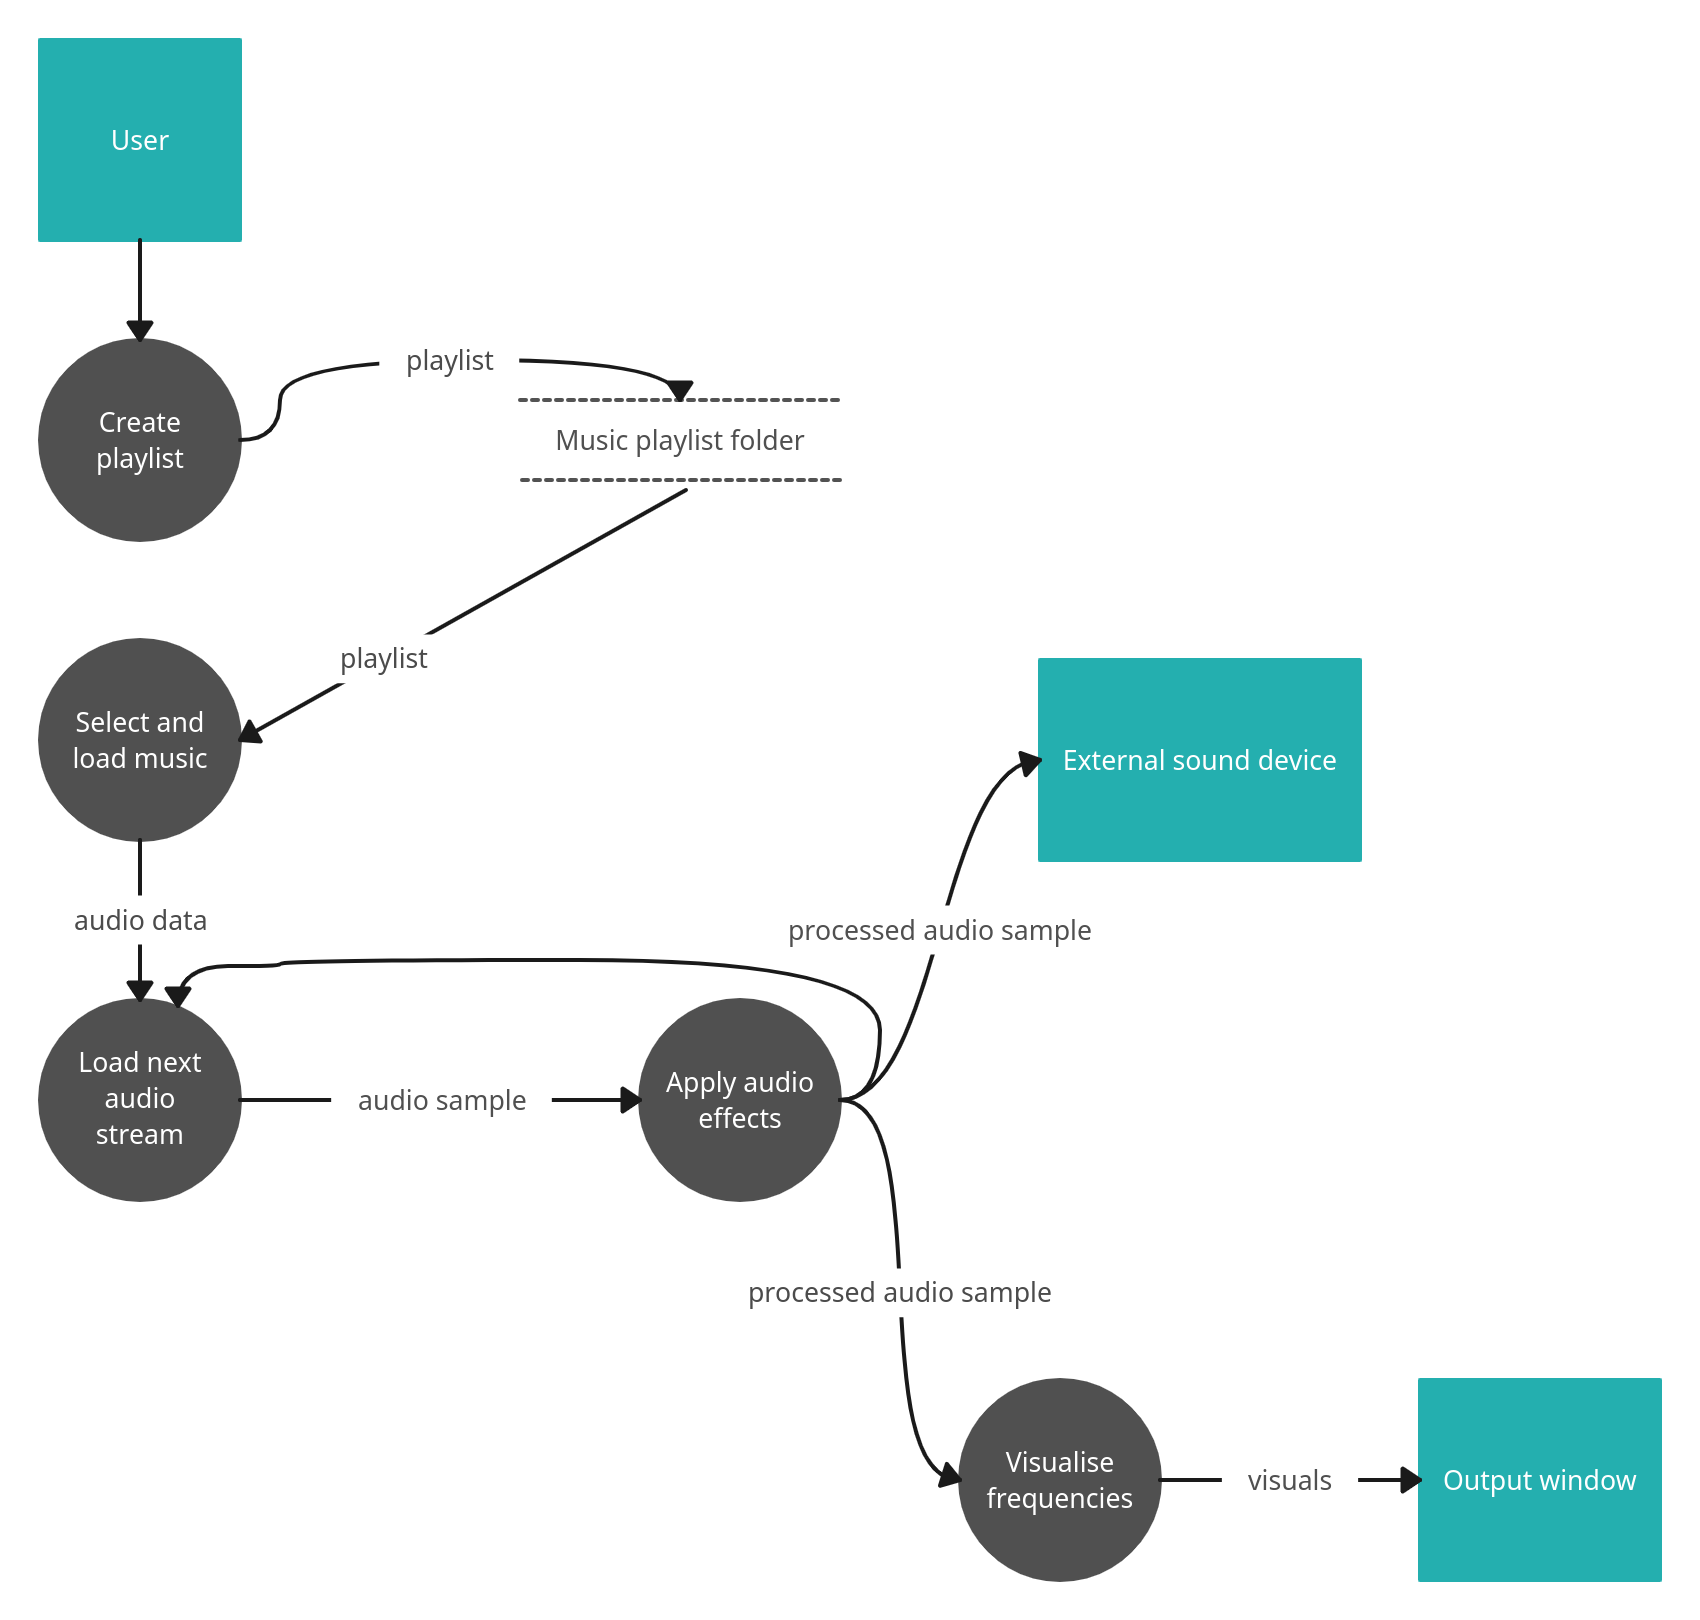
\includegraphics[width=13cm]{./DFD.png}
	\caption{The data flow diagram (DFD)}
\end{figure}

\pagebreak
\subsection{Analysis of Similar Software Products}
Every consideration must be given to the existence of other software products which may implement, either partially or fully, the features of the program yet to be implemented, in order to highlight the niche in which this project falls.

\paragraph{}
There exists two broad categories of software which provides features similar to this project:
\begin{itemize}
	\item Real-time music players - the majority of music listeners listen to music in real-time using streaming services such as Spotify or Apple Music, which can provide certain features to adjust songs in frequency-space (albeit crudely)

	\item Audio editors - for those who wish to radically alter audio (e.g. to create a remix), software such as Audacity provides many effects and processing opportunities. These are, however, "offline" in the sense that such software is not real-time.
\end{itemize}

\subsubsection{Streaming Services}
Currently within the market the two most popular music streaming products are Apple Music, with 88 million customers in 2022, and Spotify, which over 500 million. These allow users to listen to music on-demand, with both providing an "equaliser" feature that allows the user to modify the relative volume of frequencies within a song in real-time. In other words, with both these products one can, for example, alter the bass of a song, which mirrors very closely one of the main aims of this project.

\begin{figure}[H]
	\caption{The Spotify equaliser}
	\begin{center}
		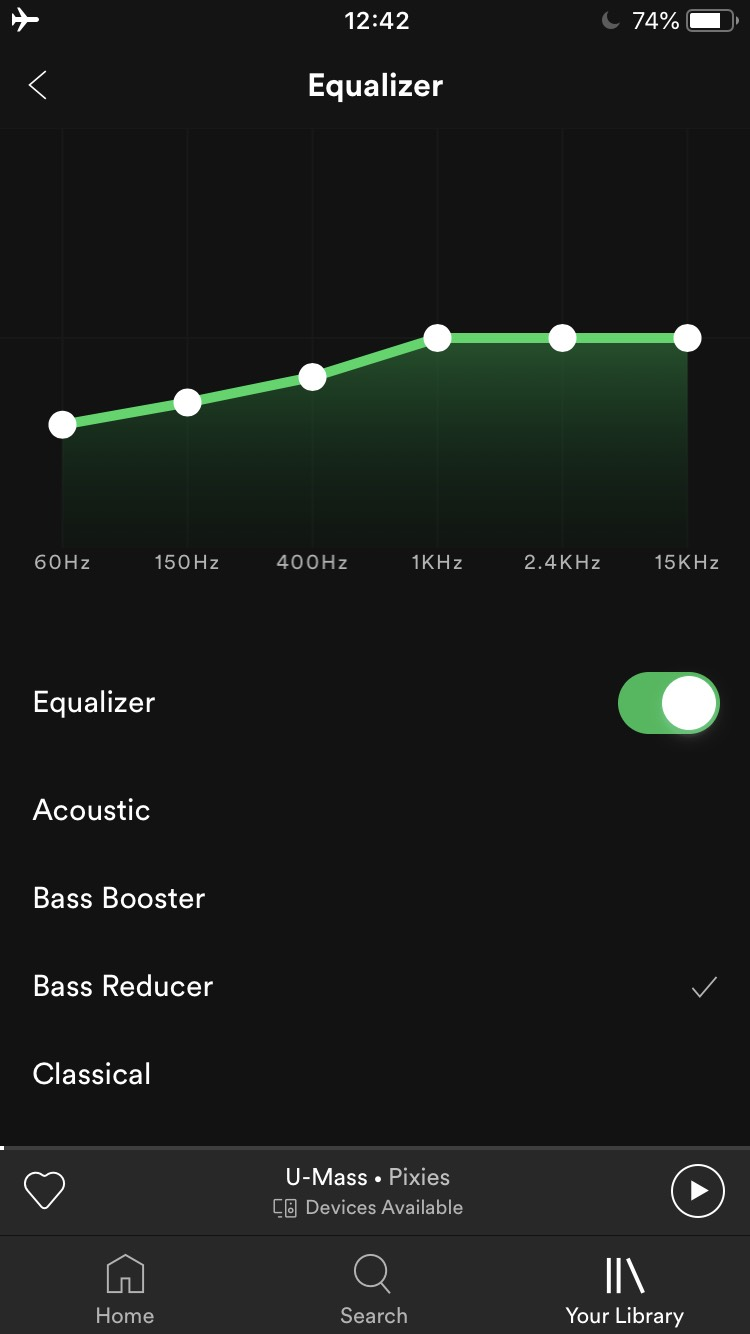
\includegraphics[width=5cm]{./spotify equaliser.jpg}
	\end{center}
\end{figure}

\begin{figure}[H]
	\caption{The Apple equaliser}
	\begin{center}
		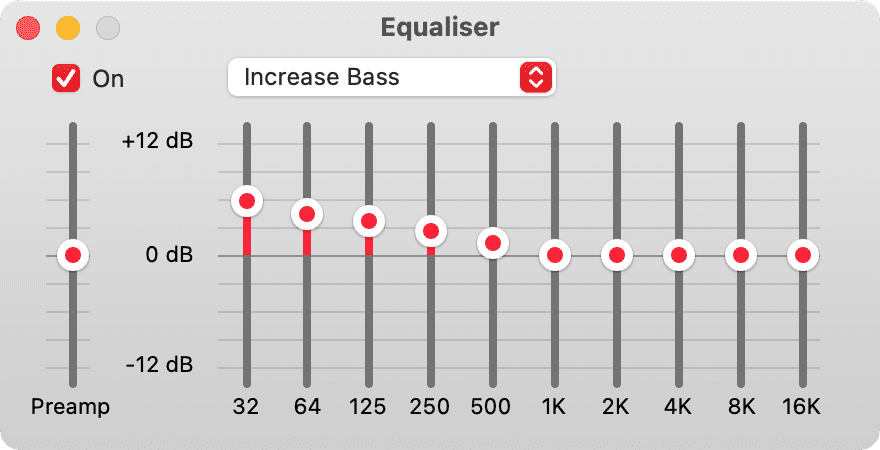
\includegraphics[width=10cm]{./apple equaliser.png}
	\end{center}
\end{figure}

As can be seen above, there are a number of similarities with the aims of this project:
\begin{itemize}
	\item The user can easily drag various points  to modify the relative volumes of a number of "frequency groups". For example, one could drag the left-most dot to its maximum height in both to boost frequencies under either 60 or 30 Hz.
	\item Ready-made "presets" can be chosen at will to assist those who may be unfamiliar with the settings presented or want to achieve a particular, pre-made effect.
	\item In Apple Music, the overall volume of the music can be adjusted.
\end{itemize}

\paragraph{}
However, there are also a few notable areas in which the two products above fall short of the features being implemented in this project, and hence fail to satisfy the needs of the users outlined in section 1.1.
\begin{itemize}
	\item In neither case does the user have exact control over the precise frequencies being modified.  If, for example, one had identified a particularly intriguing instrument playing from 500 Hz - 700 Hz, it would be impossible to isolate that frequency and boost it.
	\item There is no option to apply other audio effects such as an echo or noise. As such there are very few ways one can actually modify the audio, so creating a full "remix", that feels distinct from the original, is impossible.
\end{itemize}

\paragraph{}
Thus whilst on a surface-level, the presence of "audio equalisers" in both software products may appear to conflict with the aims of this project, especially as they perform their processing in real-time, closer inspection reveals that they offer only extremely limited options, without the ability to customise which precise frequencies are adjusted or indeed apply any other audio effects.

\subsubsection{Audio Editing Software}
On the other hand, there exists many programs which allow a user to modify audio using a great range of effects and filters. As the aim of this project is to lower the barrier of entry to creating song "remixes", it is to be free, and as such it is most worthwhile only considering other free audio editing software.

\paragraph{}
The most popular free audio editing application is Audacity, an open-source project that supports an extremely large number of effects. Additionally, it supports viewing a spectrogram of the audio being played (which visualises the audio in frequency-space just like this project aims to do), although the feature is somewhat hidden away.

\begin{figure}[H]
	\caption{Audacity when configured to display a spectrogram of the audio, seen as two multi-coloured strips (one for each channel)}
	\begin{center}
		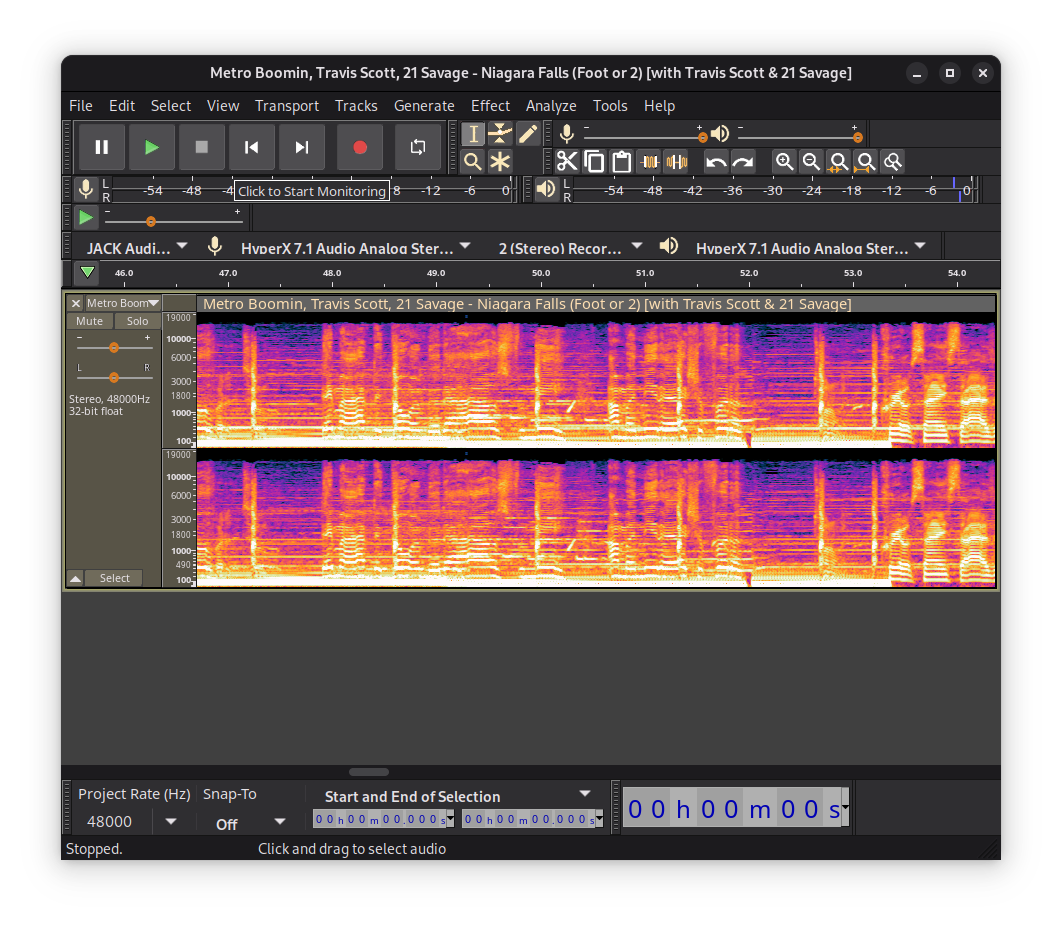
\includegraphics[width=15cm]{./audacity spectogram.png}
	\end{center}
\end{figure}

\begin{figure}[H]
	\caption{Audacity's "effects menu", offering a number of categories which themselves all contain numerous effects}
	\begin{center}
		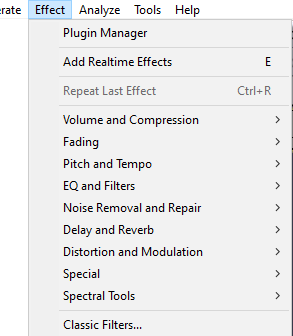
\includegraphics[width=5cm]{./audacity effects menu.png}
	\end{center}
\end{figure}

\begin{figure}[H]
	\caption{Audacity offering a menu to configure the application of a computationally-intensive, though highly accurate, reverb effect}
	\begin{center}
		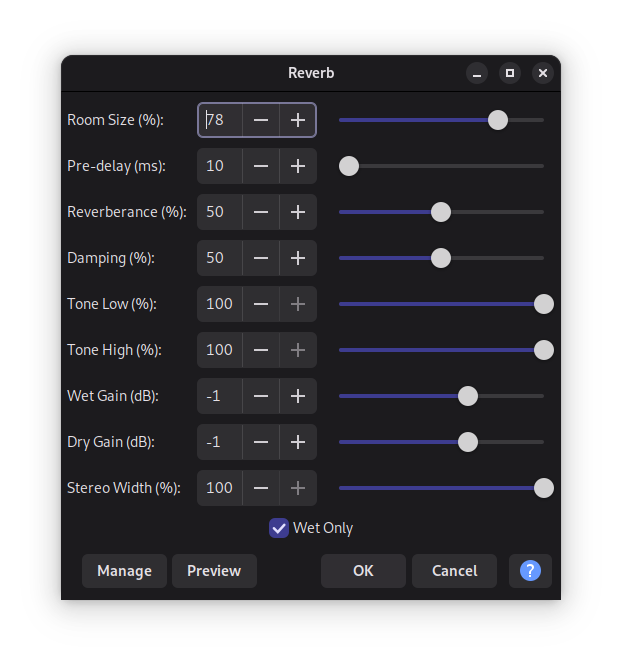
\includegraphics[width=9cm]{./audacity effects.png}
	\end{center}
\end{figure}

\paragraph{}
As can be seen above, Audacity thus presents a number of strengths which could be seen to risk overshadowing this project:
\begin{itemize}
	\item A great number of effects are supported, far greater than this project's scope could hope to provide
	\item The effects are all highly physically accurate, with extreme levels of customisation
\end{itemize}

However, its weaknesses should also be stressed:
\begin{itemize}
	\item The user interface is daunting for new users, raising the barrier of entry. For example, the process of displaying a spectrogram is not at all obvious and is hidden away.
	\item The sheer number of parameters for controlling effects is likely very daunting for people that just want a "quick remix".
	\item There are no ready-made "presets" for those too confused to immediately start applying effects themselves, or for those quickly looking for a specific modification.
	\item One cannot apply any effects in real-time, and often the effects are so computationally expensive that one must wait multiple seconds before hearing the result, even on powerful hardware.
	\item It is impossible to create a "music playlist" to listen to multiple songs in quick succession.
\end{itemize}

Hence it can be seen that whilst Audacity, and other audio editing software, provides many mechanisms for manipulating audio, it cannot be done in real-time, and often powerful hardware is required. They are also completely unsuitable as real-time music players, as they cannot play "playlists". Additionally, the sheer range of editing options would likely prove daunting to even the most experienced user, and so when one considers the high barrier of entry, the failure to be real-time, and the lack of "playlist" functionality, it is clear that audio editing programs such as Audacity do not conflict with the aims of this project.

\subsubsection{Summary of Similar Software Products}
\begin{figure}[H]
	\caption{S.W.O.T diagram for streaming services}
	\begin{center}
		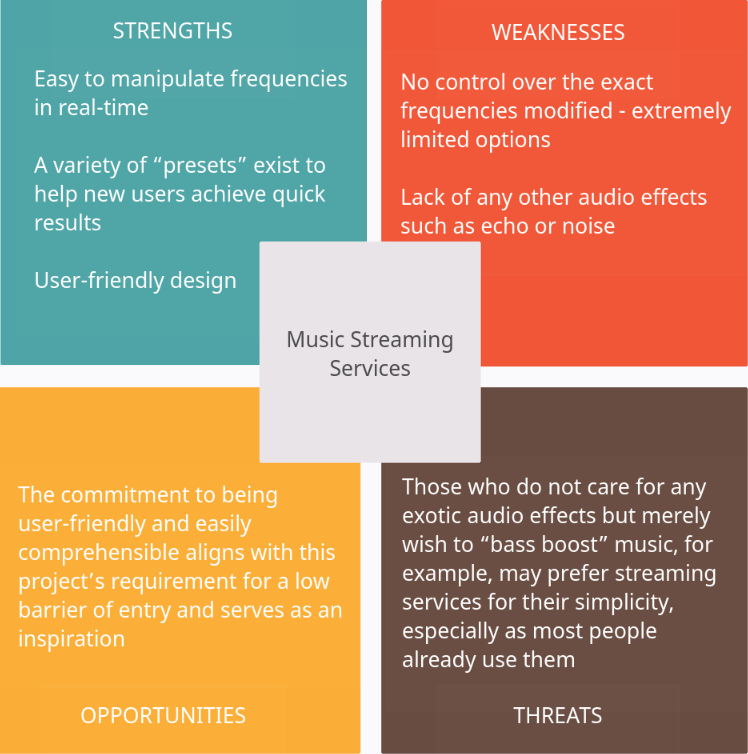
\includegraphics[width=10cm]{./SWOT streaming.png}
	\end{center}
\end{figure}
\begin{figure}[H]
	\caption{S.W.O.T diagram for audio editing prograrms}
	\begin{center}
		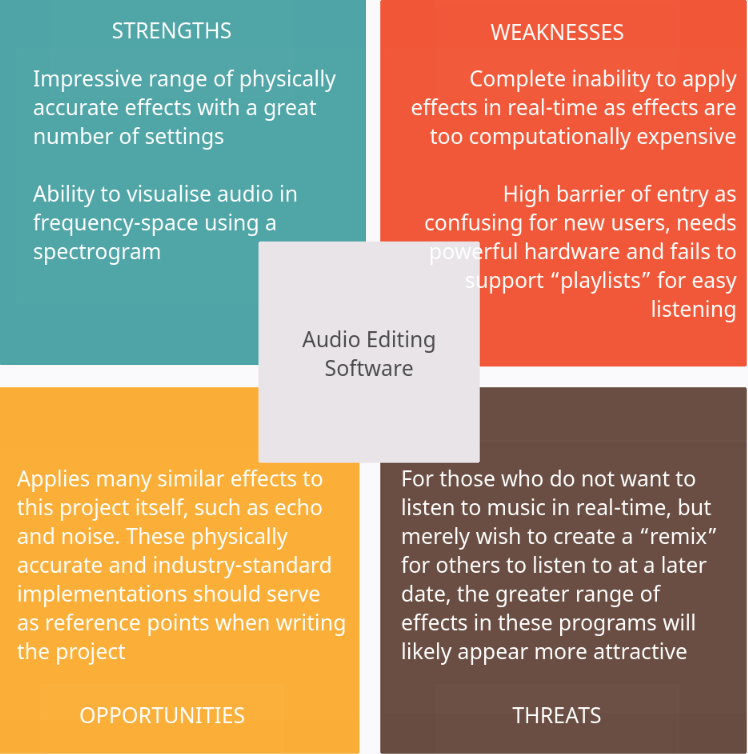
\includegraphics[width=10cm]{./SWOT audacity.png}
	\end{center}
\end{figure}

\pagebreak
\subsection{Final objectives}
\begin{enumerate}
	\item  The user must be able to load a collection of audio files known as a "playlist" and then play the audio files contained within, organised alphabetically, as is the custom in audio-listening applications.
	\item  The user must be able to visualise the current audio being played in the frequency domain (i.e. visualise the frequencies)
	\item The user must be able to modify the audio's frequency domain (i.e. selectively modify frequencies such as by reducing the bass)
	\item The user must be able to apply additional "audio effects" to further enhance the music: echo, volume adjustment and noise
	\item The user must be able to configure these "audio effects" individually, yet also apply pre-made "presets" to quickly reach a desired effect
	\item  The system must run in real-time on an average school computer
	\item The user must be able to alter the speed at which audio is played
\end{enumerate}